% Generated by ArticleSignalDiagrams. Opaque vector fills only.
\documentclass[10pt,tikz,border=5pt]{standalone}
\usepackage{lmodern}
\usetikzlibrary{fit}
\begin{document}
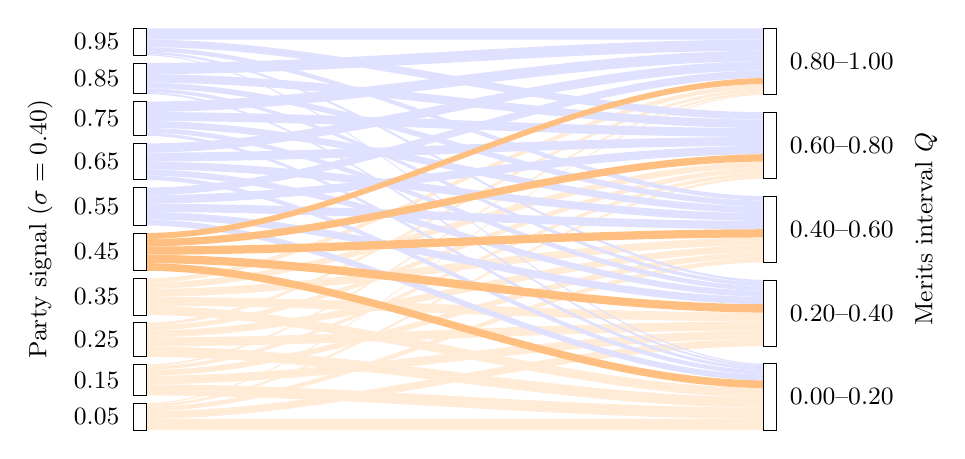
\begin{tikzpicture}[x=1cm,y=1cm,font=\small]\path[fill=orange!16!white,draw=none] (3.3,-5.1) .. controls (6,-5.1) and (8.6,-5.1) .. (11.3,-5.1) -- (11.3,-4.958346) .. controls (8.6,-4.958346) and (6,-4.958346) .. (3.3,-4.958346) -- cycle;
\path[fill=orange!16!white,draw=none] (3.3,-4.958346) .. controls (6,-4.958346) and (8.6,-4.035) .. (11.3,-4.035) -- (11.3,-3.940743) .. controls (8.6,-3.940743) and (6,-4.864089) .. (3.3,-4.864089) -- cycle;
\path[fill=orange!16!white,draw=none] (3.3,-4.864089) .. controls (6,-4.864089) and (8.6,-2.97) .. (11.3,-2.97) -- (11.3,-2.913057) .. controls (8.6,-2.913057) and (6,-4.807145) .. (3.3,-4.807145) -- cycle;
\path[fill=orange!16!white,draw=none] (3.3,-4.807145) .. controls (6,-4.807145) and (8.6,-1.905) .. (11.3,-1.905) -- (11.3,-1.873928) .. controls (8.6,-1.873928) and (6,-4.776073) .. (3.3,-4.776073) -- cycle;
\path[fill=orange!16!white,draw=none] (3.3,-4.776073) .. controls (6,-4.776073) and (8.6,-0.84) .. (11.3,-0.84) -- (11.3,-0.824621) .. controls (8.6,-0.824621) and (6,-4.760694) .. (3.3,-4.760694) -- cycle;
\path[fill=orange!16!white,draw=none] (3.3,-4.660694) .. controls (6,-4.660694) and (8.6,-4.958346) .. (11.3,-4.958346) -- (11.3,-4.817134) .. controls (8.6,-4.817134) and (6,-4.519482) .. (3.3,-4.519482) -- cycle;
\path[fill=orange!16!white,draw=none] (3.3,-4.519482) .. controls (6,-4.519482) and (8.6,-3.940743) .. (11.3,-3.940743) -- (11.3,-3.834438) .. controls (8.6,-3.834438) and (6,-4.413178) .. (3.3,-4.413178) -- cycle;
\path[fill=orange!16!white,draw=none] (3.3,-4.413178) .. controls (6,-4.413178) and (8.6,-2.913057) .. (11.3,-2.913057) -- (11.3,-2.840407) .. controls (8.6,-2.840407) and (6,-4.340528) .. (3.3,-4.340528) -- cycle;
\path[fill=orange!16!white,draw=none] (3.3,-4.340528) .. controls (6,-4.340528) and (8.6,-1.873928) .. (11.3,-1.873928) -- (11.3,-1.829084) .. controls (8.6,-1.829084) and (6,-4.295684) .. (3.3,-4.295684) -- cycle;
\path[fill=orange!16!white,draw=none] (3.3,-4.295684) .. controls (6,-4.295684) and (8.6,-0.824621) .. (11.3,-0.824621) -- (11.3,-0.799508) .. controls (8.6,-0.799508) and (6,-4.270572) .. (3.3,-4.270572) -- cycle;
\path[fill=orange!16!white,draw=none] (3.3,-4.170572) .. controls (6,-4.170572) and (8.6,-4.817134) .. (11.3,-4.817134) -- (11.3,-4.684679) .. controls (8.6,-4.684679) and (6,-4.038117) .. (3.3,-4.038117) -- cycle;
\path[fill=orange!16!white,draw=none] (3.3,-4.038117) .. controls (6,-4.038117) and (8.6,-3.834438) .. (11.3,-3.834438) -- (11.3,-3.72163) .. controls (8.6,-3.72163) and (6,-3.925309) .. (3.3,-3.925309) -- cycle;
\path[fill=orange!16!white,draw=none] (3.3,-3.925309) .. controls (6,-3.925309) and (8.6,-2.840407) .. (11.3,-2.840407) -- (11.3,-2.753196) .. controls (8.6,-2.753196) and (6,-3.838098) .. (3.3,-3.838098) -- cycle;
\path[fill=orange!16!white,draw=none] (3.3,-3.838098) .. controls (6,-3.838098) and (8.6,-1.829084) .. (11.3,-1.829084) -- (11.3,-1.768187) .. controls (8.6,-1.768187) and (6,-3.777201) .. (3.3,-3.777201) -- cycle;
\path[fill=orange!16!white,draw=none] (3.3,-3.777201) .. controls (6,-3.777201) and (8.6,-0.799508) .. (11.3,-0.799508) -- (11.3,-0.760928) .. controls (8.6,-0.760928) and (6,-3.73862) .. (3.3,-3.73862) -- cycle;
\path[fill=orange!16!white,draw=none] (3.3,-3.63862) .. controls (6,-3.63862) and (8.6,-4.684679) .. (11.3,-4.684679) -- (11.3,-4.567778) .. controls (8.6,-4.567778) and (6,-3.521719) .. (3.3,-3.521719) -- cycle;
\path[fill=orange!16!white,draw=none] (3.3,-3.521719) .. controls (6,-3.521719) and (8.6,-3.72163) .. (11.3,-3.72163) -- (11.3,-3.608993) .. controls (8.6,-3.608993) and (6,-3.409082) .. (3.3,-3.409082) -- cycle;
\path[fill=orange!16!white,draw=none] (3.3,-3.409082) .. controls (6,-3.409082) and (8.6,-2.753196) .. (11.3,-2.753196) -- (11.3,-2.65469) .. controls (8.6,-2.65469) and (6,-3.310576) .. (3.3,-3.310576) -- cycle;
\path[fill=orange!16!white,draw=none] (3.3,-3.310576) .. controls (6,-3.310576) and (8.6,-1.768187) .. (11.3,-1.768187) -- (11.3,-1.690376) .. controls (8.6,-1.690376) and (6,-3.232766) .. (3.3,-3.232766) -- cycle;
\path[fill=orange!16!white,draw=none] (3.3,-3.232766) .. controls (6,-3.232766) and (8.6,-0.760928) .. (11.3,-0.760928) -- (11.3,-0.705157) .. controls (8.6,-0.705157) and (6,-3.176995) .. (3.3,-3.176995) -- cycle;
\path[fill=blue!12!white,draw=none] (3.3,-2.5) .. controls (6,-2.5) and (8.6,-4.470699) .. (11.3,-4.470699) -- (11.3,-4.394843) .. controls (8.6,-4.394843) and (6,-2.424144) .. (3.3,-2.424144) -- cycle;
\path[fill=blue!12!white,draw=none] (3.3,-2.424144) .. controls (6,-2.424144) and (8.6,-3.503171) .. (11.3,-3.503171) -- (11.3,-3.409624) .. controls (8.6,-3.409624) and (6,-2.330597) .. (3.3,-2.330597) -- cycle;
\path[fill=blue!12!white,draw=none] (3.3,-2.330597) .. controls (6,-2.330597) and (8.6,-2.55) .. (11.3,-2.55) -- (11.3,-2.44531) .. controls (8.6,-2.44531) and (6,-2.225907) .. (3.3,-2.225907) -- cycle;
\path[fill=blue!12!white,draw=none] (3.3,-2.225907) .. controls (6,-2.225907) and (8.6,-1.596829) .. (11.3,-1.596829) -- (11.3,-1.491007) .. controls (8.6,-1.491007) and (6,-2.120084) .. (3.3,-2.120084) -- cycle;
\path[fill=blue!12!white,draw=none] (3.3,-2.120084) .. controls (6,-2.120084) and (8.6,-0.629301) .. (11.3,-0.629301) -- (11.3,-0.532222) .. controls (8.6,-0.532222) and (6,-2.023005) .. (3.3,-2.023005) -- cycle;
\path[fill=blue!12!white,draw=none] (3.3,-1.923005) .. controls (6,-1.923005) and (8.6,-4.394843) .. (11.3,-4.394843) -- (11.3,-4.339072) .. controls (8.6,-4.339072) and (6,-1.867234) .. (3.3,-1.867234) -- cycle;
\path[fill=blue!12!white,draw=none] (3.3,-1.867234) .. controls (6,-1.867234) and (8.6,-3.409624) .. (11.3,-3.409624) -- (11.3,-3.331813) .. controls (8.6,-3.331813) and (6,-1.789424) .. (3.3,-1.789424) -- cycle;
\path[fill=blue!12!white,draw=none] (3.3,-1.789424) .. controls (6,-1.789424) and (8.6,-2.44531) .. (11.3,-2.44531) -- (11.3,-2.346804) .. controls (8.6,-2.346804) and (6,-1.690918) .. (3.3,-1.690918) -- cycle;
\path[fill=blue!12!white,draw=none] (3.3,-1.690918) .. controls (6,-1.690918) and (8.6,-1.491007) .. (11.3,-1.491007) -- (11.3,-1.37837) .. controls (8.6,-1.37837) and (6,-1.578281) .. (3.3,-1.578281) -- cycle;
\path[fill=blue!12!white,draw=none] (3.3,-1.578281) .. controls (6,-1.578281) and (8.6,-0.532222) .. (11.3,-0.532222) -- (11.3,-0.415321) .. controls (8.6,-0.415321) and (6,-1.46138) .. (3.3,-1.46138) -- cycle;
\path[fill=blue!12!white,draw=none] (3.3,-1.36138) .. controls (6,-1.36138) and (8.6,-4.339072) .. (11.3,-4.339072) -- (11.3,-4.300492) .. controls (8.6,-4.300492) and (6,-1.322799) .. (3.3,-1.322799) -- cycle;
\path[fill=blue!12!white,draw=none] (3.3,-1.322799) .. controls (6,-1.322799) and (8.6,-3.331813) .. (11.3,-3.331813) -- (11.3,-3.270916) .. controls (8.6,-3.270916) and (6,-1.261902) .. (3.3,-1.261902) -- cycle;
\path[fill=blue!12!white,draw=none] (3.3,-1.261902) .. controls (6,-1.261902) and (8.6,-2.346804) .. (11.3,-2.346804) -- (11.3,-2.259593) .. controls (8.6,-2.259593) and (6,-1.174691) .. (3.3,-1.174691) -- cycle;
\path[fill=blue!12!white,draw=none] (3.3,-1.174691) .. controls (6,-1.174691) and (8.6,-1.37837) .. (11.3,-1.37837) -- (11.3,-1.265562) .. controls (8.6,-1.265562) and (6,-1.061883) .. (3.3,-1.061883) -- cycle;
\path[fill=blue!12!white,draw=none] (3.3,-1.061883) .. controls (6,-1.061883) and (8.6,-0.415321) .. (11.3,-0.415321) -- (11.3,-0.282866) .. controls (8.6,-0.282866) and (6,-0.929428) .. (3.3,-0.929428) -- cycle;
\path[fill=blue!12!white,draw=none] (3.3,-0.829428) .. controls (6,-0.829428) and (8.6,-4.300492) .. (11.3,-4.300492) -- (11.3,-4.275379) .. controls (8.6,-4.275379) and (6,-0.804316) .. (3.3,-0.804316) -- cycle;
\path[fill=blue!12!white,draw=none] (3.3,-0.804316) .. controls (6,-0.804316) and (8.6,-3.270916) .. (11.3,-3.270916) -- (11.3,-3.226072) .. controls (8.6,-3.226072) and (6,-0.759472) .. (3.3,-0.759472) -- cycle;
\path[fill=blue!12!white,draw=none] (3.3,-0.759472) .. controls (6,-0.759472) and (8.6,-2.259593) .. (11.3,-2.259593) -- (11.3,-2.186943) .. controls (8.6,-2.186943) and (6,-0.686822) .. (3.3,-0.686822) -- cycle;
\path[fill=blue!12!white,draw=none] (3.3,-0.686822) .. controls (6,-0.686822) and (8.6,-1.265562) .. (11.3,-1.265562) -- (11.3,-1.159257) .. controls (8.6,-1.159257) and (6,-0.580518) .. (3.3,-0.580518) -- cycle;
\path[fill=blue!12!white,draw=none] (3.3,-0.580518) .. controls (6,-0.580518) and (8.6,-0.282866) .. (11.3,-0.282866) -- (11.3,-0.141654) .. controls (8.6,-0.141654) and (6,-0.439306) .. (3.3,-0.439306) -- cycle;
\path[fill=blue!12!white,draw=none] (3.3,-0.339306) .. controls (6,-0.339306) and (8.6,-4.275379) .. (11.3,-4.275379) -- (11.3,-4.26) .. controls (8.6,-4.26) and (6,-0.323927) .. (3.3,-0.323927) -- cycle;
\path[fill=blue!12!white,draw=none] (3.3,-0.323927) .. controls (6,-0.323927) and (8.6,-3.226072) .. (11.3,-3.226072) -- (11.3,-3.195) .. controls (8.6,-3.195) and (6,-0.292855) .. (3.3,-0.292855) -- cycle;
\path[fill=blue!12!white,draw=none] (3.3,-0.292855) .. controls (6,-0.292855) and (8.6,-2.186943) .. (11.3,-2.186943) -- (11.3,-2.13) .. controls (8.6,-2.13) and (6,-0.235911) .. (3.3,-0.235911) -- cycle;
\path[fill=blue!12!white,draw=none] (3.3,-0.235911) .. controls (6,-0.235911) and (8.6,-1.159257) .. (11.3,-1.159257) -- (11.3,-1.065) .. controls (8.6,-1.065) and (6,-0.141654) .. (3.3,-0.141654) -- cycle;
\path[fill=blue!12!white,draw=none] (3.3,-0.141654) .. controls (6,-0.141654) and (8.6,-0.141654) .. (11.3,-0.141654) -- (11.3,0) .. controls (8.6,0) and (6,-0) .. (3.3,-0) -- cycle;
\path[fill=orange!50!white,draw=none] (3.3,-3.076995) .. controls (6,-3.076995) and (8.6,-4.567778) .. (11.3,-4.567778) -- (11.3,-4.470699) .. controls (8.6,-4.470699) and (6,-2.979916) .. (3.3,-2.979916) -- cycle;
\path[fill=orange!50!white,draw=none] (3.3,-2.979916) .. controls (6,-2.979916) and (8.6,-3.608993) .. (11.3,-3.608993) -- (11.3,-3.503171) .. controls (8.6,-3.503171) and (6,-2.874093) .. (3.3,-2.874093) -- cycle;
\path[fill=orange!50!white,draw=none] (3.3,-2.874093) .. controls (6,-2.874093) and (8.6,-2.65469) .. (11.3,-2.65469) -- (11.3,-2.55) .. controls (8.6,-2.55) and (6,-2.769403) .. (3.3,-2.769403) -- cycle;
\path[fill=orange!50!white,draw=none] (3.3,-2.769403) .. controls (6,-2.769403) and (8.6,-1.690376) .. (11.3,-1.690376) -- (11.3,-1.596829) .. controls (8.6,-1.596829) and (6,-2.675856) .. (3.3,-2.675856) -- cycle;
\path[fill=orange!50!white,draw=none] (3.3,-2.675856) .. controls (6,-2.675856) and (8.6,-0.705157) .. (11.3,-0.705157) -- (11.3,-0.629301) .. controls (8.6,-0.629301) and (6,-2.6) .. (3.3,-2.6) -- cycle;
\coordinate (axis-midline-0) at (0,-2.55);
\path[fill=white,draw=black,line width=0.3pt] (3.22,-5.1) rectangle (3.38,-4.760694);
\node[anchor=east,fill=white,inner sep=2pt] (bucket-0-0-0) at (3.12,-4.930347) {0.05};
\path[fill=white,draw=black,line width=0.3pt] (3.22,-4.660694) rectangle (3.38,-4.270572);
\node[anchor=east,fill=white,inner sep=2pt] (bucket-0-0-1) at (3.12,-4.465633) {0.15};
\path[fill=white,draw=black,line width=0.3pt] (3.22,-4.170572) rectangle (3.38,-3.73862);
\node[anchor=east,fill=white,inner sep=2pt] (bucket-0-0-2) at (3.12,-3.954596) {0.25};
\path[fill=white,draw=black,line width=0.3pt] (3.22,-3.63862) rectangle (3.38,-3.176995);
\node[anchor=east,fill=white,inner sep=2pt] (bucket-0-0-3) at (3.12,-3.407808) {0.35};
\path[fill=white,draw=black,line width=0.3pt] (3.22,-3.076995) rectangle (3.38,-2.6);
\node[anchor=east,fill=white,inner sep=2pt] (bucket-0-0-4) at (3.12,-2.838498) {0.45};
\path[fill=white,draw=black,line width=0.3pt] (3.22,-2.5) rectangle (3.38,-2.023005);
\node[anchor=east,fill=white,inner sep=2pt] (bucket-0-0-5) at (3.12,-2.261502) {0.55};
\path[fill=white,draw=black,line width=0.3pt] (3.22,-1.923005) rectangle (3.38,-1.46138);
\node[anchor=east,fill=white,inner sep=2pt] (bucket-0-0-6) at (3.12,-1.692192) {0.65};
\path[fill=white,draw=black,line width=0.3pt] (3.22,-1.36138) rectangle (3.38,-0.929428);
\node[anchor=east,fill=white,inner sep=2pt] (bucket-0-0-7) at (3.12,-1.145404) {0.75};
\path[fill=white,draw=black,line width=0.3pt] (3.22,-0.829428) rectangle (3.38,-0.439306);
\node[anchor=east,fill=white,inner sep=2pt] (bucket-0-0-8) at (3.12,-0.634367) {0.85};
\path[fill=white,draw=black,line width=0.3pt] (3.22,-0.339306) rectangle (3.38,-0);
\node[anchor=east,fill=white,inner sep=2pt] (bucket-0-0-9) at (3.12,-0.169653) {0.95};
\node[fit=(bucket-0-0-0) (bucket-0-0-1) (bucket-0-0-2) (bucket-0-0-3) (bucket-0-0-4) (bucket-0-0-5) (bucket-0-0-6) (bucket-0-0-7) (bucket-0-0-8) (bucket-0-0-9),inner sep=0pt] (source-labels-0) {};
\coordinate (axis-title-0-0) at (source-labels-0.west |- axis-midline-0);
\node[rotate=90,anchor=south,inner sep=0pt] at ([xshift=-0.18cm]axis-title-0-0) {Party signal ($\sigma=0.40$)};
\path[fill=white,draw=black,line width=0.3pt] (11.22,-5.1) rectangle (11.38,-4.26);
\node[anchor=west,fill=white,inner sep=2pt] (bucket-0-1-0) at (11.48,-4.68) {0.00--0.20};
\path[fill=white,draw=black,line width=0.3pt] (11.22,-4.035) rectangle (11.38,-3.195);
\node[anchor=west,fill=white,inner sep=2pt] (bucket-0-1-1) at (11.48,-3.615) {0.20--0.40};
\path[fill=white,draw=black,line width=0.3pt] (11.22,-2.97) rectangle (11.38,-2.13);
\node[anchor=west,fill=white,inner sep=2pt] (bucket-0-1-2) at (11.48,-2.55) {0.40--0.60};
\path[fill=white,draw=black,line width=0.3pt] (11.22,-1.905) rectangle (11.38,-1.065);
\node[anchor=west,fill=white,inner sep=2pt] (bucket-0-1-3) at (11.48,-1.485) {0.60--0.80};
\path[fill=white,draw=black,line width=0.3pt] (11.22,-0.84) rectangle (11.38,0);
\node[anchor=west,fill=white,inner sep=2pt] (bucket-0-1-4) at (11.48,-0.42) {0.80--1.00};
\node[fit=(bucket-0-1-0) (bucket-0-1-1) (bucket-0-1-2) (bucket-0-1-3) (bucket-0-1-4),inner sep=0pt] (destination-labels-0) {};
\coordinate (axis-title-0-1) at (destination-labels-0.east |- axis-midline-0);
\node[rotate=90,anchor=north,inner sep=0pt] at ([xshift=0.18cm]axis-title-0-1) {Merits interval $Q$};
\end{tikzpicture}
\end{document}

